\documentclass[a4paper]{scrreprt}

\usepackage[ngerman]{babel}   % deutsche Silbentrennung

\usepackage[utf8x]{inputenc}
\usepackage[T1]{fontenc}
\usepackage{lmodern}			% Schönere Schriftart		
\usepackage{hyperref}

%\usepackage[ansinew]{inputenc}
%\usepackage[utf8]{inputenc}   % wegen deutschen Umlauten & UTF-8

\usepackage{graphicx}					% Grafikpaket laden
\usepackage{svg}
\usepackage{hyperref}					% Links
\hypersetup{									% Link-Formatierung entfernen & pdf-Inforamtionen setzten
	pdfauthor={Grigori Schapoval, Nathanael Schneider, Tim Brodbeck, Stefan Wolf, Jens Manig, Laurenz Thiel},
	pdftitle={3D Reconstruction Framework from Multi-View Images (3D-MuVi)},
	colorlinks,
	citecolor=black,
	filecolor=black,
	linkcolor=black,
	urlcolor=black
}
%\usepackage{microtype}		% font expansion
\usepackage{enumerate}
\usepackage{xstring}
\usepackage{enumitem}    % Layout der Aufzählungs-Items manipulieren
\setlist{nosep}
\usepackage[ngerman]{cleveref}
\title{Praxis der Softwareentwicklung:\\3D Reconstruction Framework from Multi-View Images (3D-MuVi)}
\subtitle{Entwurfsdokument}
\author{Grigori Schapoval\and Nathanael Schneider\and Tim Brodbeck\and Stefan Wolf\and Jens Manig\and Laurenz Thiel}
\date{
\includegraphics[width=.3\textwidth]{img/logo.pdf}\\\vspace{3mm}WS 2015/16}


% Ein paar makros (Nathanael)
%% Liste ein paar Methoden auf
\newcommand{\beginMembers}{~\\ \textbf{Methoden:} \begin{itemize} }
%% Liste ein paar Slots auf
\newcommand{\beginSlots}{~\\ \textbf{Slots:} \begin{itemize} }
%% Liste ein paar einzelne Attribute auf
\newcommand{\beginAttributes}{~\\ \textbf{Attribute:} \begin{itemize} }
	
\newcommand{\beginSignals}{~\\ \textbf{Signale:} \begin{itemize} }
%% Ein neuer Member. Zuerst Name, dann Argumente + evtl Docs, Dann rückgabe, dann beschreibung
\newcommand{\newMember}[4] {\item \textbf{#1} \\ #4 \\Übergabeparameter: #2 \\ Rückgabetyp: #3}
%% Ein neuer Slot. Zuerst name, dann passendes Signal, dann beschreibung
\newcommand{\newSlot}[3]{\item \textbf{#1} \\ #3 \\Signal: #2}
%% Ein neues Signal. Zuerst name, dann parameter, dann beschreibung
\newcommand{\newSignal}[3]{\item \textbf{#1} \\ #3 \\Übergabeparameter: #2 \\ Rückgabetyp: Signal}
%% Ein neues Attribut. Zuerst Name inkl Typ, dann beschreibung
\newcommand{\newAttribute}[2]{ \item \textbf{#1} \\ #2}
%% Ein neuer Abstrakter Member. Siehe \newMember
\newcommand{\newMemberAbstract}[4]{\item \textbf{\textit{#1}} \\ #4 \\Übergabeparameter: #2 \\ Rückgabetyp: #3}
%% Ein neuer Statischer Member. Siehe \newMember
\newcommand{\newMemberStatic}[4]{\item \underline{\textit{#1}} \\ #4 \\Übergabeparameter: #2 \\ Rückgabetyp: #3}
%% Beendet die Memberdeklaration
\newcommand{\closeMembers}{\end{itemize} }
\begin{document}
	\maketitle
	\setcounter{tocdepth}{1}
	\tableofcontents
	\chapter{Einleitung}
		% vollständige Beschreibung der Aufgabenstellung.
Die Welt wird digital - und mit ihr viele Prozesse. Die Kommunikation läuft heutzutage größtenteils mit digitalen Hilfsmitteln. Auch Geschäftsprozesse werden immer mehr Digital abgewickelt, soweit möglich. Um dies zu bewerkstelligen, müssen die Daten aus der Realen Welt allerdings erstmal digitalisiert werden. Viel ist in dieser Richtung geschehen, wie z.B. Kameras, die Digitalisierung ganzer Bibliotheken und das erfassen von Echtzeitdaten über Sensornetze sind nur ein Bruchteil. Doch das einlesen komplexer Daten ist bis heute ein nicht-triviales Problem.

Viele Arbeitsbereiche erfordern eine Speicherung und Übertragung von Daten, wie sie im echten Leben vorzufinden sind - z.B. Dreidimensionale Bilder. In der Medizin werden sie benutzt, um Knochen und Skelette platzsparend verfügbar zu haben, in der Automobilindustrie benötigt man sie, um Prototypen schon vor dem ersten tatsächlichen Fertigungsschritt vor Augen zu haben. Besonders die Spielindustrie steigert ihre Anforderungen nach immer besseren und realistischeren Modellen.

Für viele dieser Anforderungen gibt es eine einfach erscheinende Lösung. Man nehme ein reales Objekt und digitalisiere seinen dreidimensionalen Aufbau. Doch leider ist das Problem nicht so einfach, wie es sich zuerst anhört. Es gibt viele verschiedene Verfahren um diese Aufgabenstellung und jedes einzelne bewährt sich besonders in einem spezifischen Problemfeld. Ein Beispiel ist Motion Capture, das besonders für die Rekonstruktion von Bewegungen im Dreidimensionalen Raum über die Zeit genutzt wird, Laserscanner können schnell und zuverlässig Personen vermessen. Dieses Projekt beschäftigt sich gezielt mit der Rekonstruktion von digitalen Repräsentationen der Objekte über zweidimensionale Aufnahmen des gewünschten Gegenstandes oder einer kompletten Szene.

Die für den Prozess verwendeten Algorithmen sind jedoch sehr spezialisiert und decken meist nur einen bestimmten Anwendungsfall ab. Zudem lassen sich für die einzelnen Schritte auch unterschiedliche Algorithmen kombinieren, was die Zusammenstellung für ein perfektes Ergebnis umso schwerer macht. So macht es z.B. einen Unterschied, ob man eine Szene aus einem Videoclip rekonstruieren möchte, ob man einzelne Fotos aus verschiedenen Blickrichtungen hat oder ob es sich um eine Luftaufnahme handelt.

Ziel des 3D-MuVi Projekts ist es, die Kombination von Algorithmen und das damit verbundene Suchen nach dem bestmöglichen Ergebnis zu vereinfachen. Der Benutzer bekommt die Möglichkeit, verschiedene Algorithmen für die einzelnen Schritte auszuwählen und sich die Ergebnisse anzusehen, um somit das bestmögliche Resultat zu erzielen.
	\chapter{Zielbestimmung}
		% Beschreibung der Funktionalität der zu entwickelnden Systemkomponente. 
% o Musskriterien: Mindestanforderungen. 
% o Kannkriterien: Zusätzliche Funktionalität. 
% o Abgrenzungskriterien: Was gehört nicht zum Funktionsumfang? (vgl. auch Produkteinsatz) 

$\section{Abgrenzungskriterien}
Das Ziel dieses Projektes ist die Entwicklung eines Frameworks. Dieses Framework soll in der Lage sein, vorderfinierte Workflows mit ausgewählten Algorithmen zu verwenden, um eine 3D Konstruktion zu erstellen. \textit{Die Algorithmen selbst sind nicht Teil des Projekts und werden bereitgestellt.} Die notwendigen Schnittstellen für die Workflow und Algorithmen sind sicherzustellen. \newline
Falls eine Workflowkonfiguration gewählt wurde und die Berechnung gestartet ist, ist es nicht mehr möglich, Veränderungen in den Workflowkonfiigurationen vorzunehmen. Alle Einstellungen sind \textit{vor} Beginn der Berechnung feszulegen. Beim vorzeitigen, manuellen Abbruch wird nicht sichergestellt, dass die bis zu den Punkt berechneten Daten verwendbar sind. \newline
Das Framework soll eine 3D Konstruktion mithilfe eines Workflows mit Workflowkonfigurationen erstellen. Dazu steht standardgemäß ein 4-Phasen-Workflow bestehend aus Feature Extraktion / Matching, Posenschätzung, Tiefenschätzung und 3D Fusion zur Verfügung. Je nach Realisierbarkeit können auch andere Workflows in Betracht gezogen werden.
Jeder Algorithmus des Workflows braucht ggf. als Eingabe das Ergebnis eines anderen Teilschritts des Workflows. So kann es sein dass die Posenschätzung Extraktion / Matching braucht, die Tiefenschätzung die Posenschätzung usw.
Diese Abhängigkeiten erschweren die Realisierung eines dynmischen Workflowbuilders. 

\section{Lösungsansatz}
Die Benutzeroberfläche wird nur auf englischer Sprache umgesetzt. \newline
Das Framework wird erst auf eine festgelegte Anzahl an Algorithmen getestet und sichergestellt, dass der 4-Phasen-Workflow mit diesen Algorithmen funktioniert. Idealerweise sollte es später den Benutzer möglich sein die Algorithmenbibliothek selbständig erweitern können. Dabei sollte man auf die Ein- und Ausgabe der Algorithmen beachten. \newline
Beim vorzeitigen Abgebrochen ist es unter Umständen schwierig brauchbare Daten von unbrauchbaren zu trennen. Deshalb wird erstmal darauf geachtet, dass es möglich ist, überhaupt den Prozess sicher zu beenden, dass keine unbrauchbare Artefakte entstehen. Optional sollten dann, falls ALgorithmen ihre Berechnungen auf kompletten Datensatz berechnet haben, das Ergebnis der Algorithmen als Zwischenergebnis zu speichern.
\newline Außerdem werden fest definierte Workflows erstellt, um Probleme mit unrealisierbaren Workflows zu vermeiden. $

\section{Problemabgrenzung}
Aus einer Menge von Bildern eines Objektes wie z.B. eines Gebäudes soll eine digitale 3D-Rekonstruktion berechnet werden.\newline
Da es keinen einzelnen Algorithmus gibt, der für dieses Problem eine gute Lösung bietet werden Algorithmen der Feature Extraktion / Matching, der Posenschätzung, der Tiefenschätzung und 3D Fusion kombiniert und parametrisiert. Die Kombinationen der Algorithmen ergeben einen mehrstufigen Worfklow. Wenn nun eine solche Kombination von Algorithmen getestet wird, ist es erforderlich die Eingangsdaten und Parameter pro Algorithmus manuell einzustellen, um sie auszuführen. Anschließend muss mit spezieller Software das entstandene 3D-Modell visualisiert werden, um die Ergebnisse validieren zu können.\newline
Diese Umstände resultieren in einem wenig intuitiven und effektiven Umfeld zur Testung von Workflows.

\section{Lösungsansatz}
Um diesen zähen Prozess zu beschleunigen, soll ein Framework entwickelt werden, das den Großteil der Schritte automatisiert, wodurch der Anwender sich lediglich um die Komposition und Konfiguration der Algorithmen kümmern muss. Dazu sollen zunächst Bilder geladen werden können, die anschließend mit dem Start des Workflows an diesen übergeben werden. Dieser Workflow ist in Verarbeitungsschritte unterteilt, die als Plugins geladen und anschließend schnell ausgetauscht und konfiguriert werden können. Die daraus entstanden Workflow-Konfiugrationen können gespeichert und geladen werden, um z.B. ein Testen des Workflows auf eine anderen Bildermenge zu einem späteren Zeitpunkt zu erleichtern. Abschließend sollen die Ergebnisse im Programm visualisiert werden.
	\chapter{Anforderungen}
		
\section{Musskriterien}
\subsection{Modul: Workflow}
Die Software soll einen standardisierten 4-Phasen-Workflow bereitstellen, bestehend aus:

\begin{enumerate}
		\item Feature Extraktion / Matching
		\item Posenschätzung
		\item Tiefenschätzung
		\item 3D Fusion
\end{enumerate}
Für jede Phase dieses Workflows sollen verschiedene Algorithmen ausgewählt werden können.
%\begin{itemize}
%	\item Die Software soll einen standardisierten 4-Phase-Workflow bereitstellen, bestehend aus:
%	\begin{enumerate}
%		\item Feature Extraktion / Matching
%		\item Posenschätzung
%		\item Tiefenschätzung
%		\item 3D Fusion
%	\end{enumerate}
%	\item Für jede Phase dieses Workflows sollen verschiedene Algorithmen ausgewählt werden können.
%\end{itemize}
\subsection{Modul: Input/Output}
Das Programm soll eine Menge von Einzelbildern einlesen und diese an die Algorithmen zur Bearbeitung übergeben. Außerdem muss es möglich sein, die Ergebnisse bzw. Zwischenergebnisse abzuspeichern.
%\begin{itemize}
%	\item Das Programm soll eine Menge von Einzelbildern einlesen und diese an die Algorithmen zur Bearbeitung übergeben können.
%	\item Ergebnisse bzw. Zwischenergebnisse sollen gespeichert werden können.
%\end{itemize}
\subsection{Modul: Visualisierung}
Nach dem Ausführen des Workflows sind die Ergebnisse auf verschiedene Arten darstellbar. So lässt sich zum Beispiel das berechnete 3D Modell als Point Cloud visualisieren. In dieses Modell sollen Kameraposen und -orientierungen als Kamerapyramide eingezeichnet werden können. Des Weiteren soll eine Tiefenkarte der Ergebnisse als Visualisierung zur Verfügung stehen. Zuletzt soll es eine Ansicht geben, in der die berechneten Features, die durch die Algorithmen erkannt wurden, in Einzelbildern eingezeichnet sind. 
%Darstellung der Ergebnisse:
%\begin{itemize}
%	\item Features die durch die Algorithmen erkannt wurden, sollen in Einzelbildern eingezeichnet werden.
%	\item Kameraposen und -orientierungen sollen im 3D Modell als Kamerapyramide eingezeichnet werden .
%	\item Anzeigen der Tiefenkarten
%	\item Anzeige des 3D Modells als Piont Cloud.
%\end{itemize}
\subsection{Modul: Logger}
Informationen, Warnungen, Fehler und Debugmeldungen, die von den Algorithmen ausgeworfen werden, soll das Programm aufzeichnen, anzeigen und abspeichern können.
\subsection{Modul: Einstellungen}
Die Einstellungen der einzelnen Verfahren können abgespeichert und geladen werden.
\subsection{Modul: Interaktion}
Der Workflow soll gestartet und gestoppt werden können.\\Das Stoppen der Verarbeitung bewirkt, dass keine Daten weitergegeben werden und lediglich die restliche Berechnung der Workflowstufe ausgeführt wird. Zudem soll ein globaler Arbeitsindikator die andauernde Verarbeitung der Verfahren anzeigen.
%\begin{itemize}
%	\item Der Workflow soll gestartet und gestoppt werden können.\\Das Stoppen der Verarbeitung bewirkt, dass keine Daten weitergegeben werden und lediglich die restliche Berechnung der Workflowstufe ausgeführt wird.
%	\item Ein globaler Arbeitsindikator soll die andauernde Verarbeitung der Verfahren anzeigen.
%\end{itemize}

\section{Kannkriterien}
\subsection{Modul: Workflow}
Zu dem bereits existierenden 4-Phasen-Workflow sollen weitere fest implementierte Workflows zu Verfügung stehen. Die Konfiguration dieser Workflows soll abgespeichert und geladen werden können. Zusätzlich soll es möglich sein, Workflows dynamisch zu erstellen und zu verändern. 
%\begin{itemize}
%	\item Es sollen mehrere fest implementierte Workflows zu Verfügung stehen.
%	\item Workflows können variable erstellt und verändert werden.
%	\item Abspeichern und laden der Workflow-Konfiguration.
%\end{itemize}
\subsection{Modul: Visualisierung}
Neben der Point Cloud als Darstellungsvariante gibt es die Möglichkeit das 3D Modell als Mesh bzw. texturiert zu visualisieren.
%\begin{itemize}
%	\item Darstellung des 3D Modells in Form von Point Cloud, Mesh und Texturiert.
%\end{itemize}
\subsection{Modul: Einstellungen}
Die globalen Einstellungen des Programms können abgespeichert und geladen werden.
\subsection{Modul: Interaktion}
Beim Programmstart können die Workflow-Konfiguration und das Verzeichnis mit den Eingangsdaten als Commandline-Optionen übergeben werden. Außerdem soll es möglich sein, einzelne Ausführungsstufe des Workflows separat zu startet und die dafür benötigten Daten aus z.B. Ergebnisse und Zwischenergebnisse vorangegangener Berechnungen zu laden. Jede dieser Ausführungsstufen soll einen eigenen Arbeitsindikator erhalten. Zudem soll das Programm die Funktion bieten, Daten neu zu sortieren und den Workflow auf Untergruppen der Daten anzuwenden. Auch das wiederholte Ausführung von einzelnen Workflow-Stufen auf verschiedene Datensätze soll zu Verfügung stehen. Zuletzt soll bei Bedarf eine Interaktion mit den Ergebnisse und Zwischenergebnisse, wie z.B. das Bearbeiten der Kameras, Ein-, Ausblenden und Entfernen einzelner Punkte möglich sein.
%\begin{itemize}
%	\item Auswahl der Workflow-Konfiguration und Verzeichnis mit Eingangsdaten durch Commandline-Optionen beim Programmstart.	
%	\item Laden vorhergegangener (Zwischen-) Ergebnisse.
%	\item Einzelne Schritte sollen gestartet werden können.
%	\item Arbeitsindikatoren für jeden einzelnen Verarbeitungsschritt.
%	\item Daten neu Sortieren / Ausführen auf Untergruppen der Daten.
%	\item Automatisierte wiederholte Ausführung von einzelnen Algorithmen auf verschiedenen Datensätze.
%	\item Manipulation und Interaktion mit (Zwischen-) Ergebnisse.\\(z.B. Ein-, Ausblenden und Entfernen einzelner Punkte, Kameras, Matches etc.).
%\end{itemize}

\section{Abgrenzungskriterien}
\begin{itemize}
	\item Videos liegen als sortierte Einzelbilder vor.
	\item Algorithmen müssen nicht Implementiert werden. (Bereitstellung von Schnittstellen zur Einbindung)
	\item Eine Änderung der Eingabe erfordert eine erneute Ausführung der Algorithmen.
	\item Die Benutzeroberfläche beschränkt sich auf englisch Sprache.
\end{itemize}
	\chapter{Produkteinsatz}
		% Beschreibt  Einsatzgebiete,  Zielgruppe  und  Betriebsbedingungen  sowie  notwendige Hard‐ und Software.
\section{Einsatzgebiet}
\section{Anwendungsbereich}
\section{Zielgruppe}
\section{Betriebsbedingungen} 

	\chapter{Produktumgebung}
		% Notwendige Hard‐ und Software.
\section{Software}
Das Programm soll auf linuxbasierten Betriebssystemen laufen, da es mit QT entwickelt und möglichst Plattform unabhängig entwickelt wird, kann es sein, dass es auch unter anderen Betriebssystemen läuft.
\section{Hardware}
Als Hardware wird ein einfacher PC benötigt, welcher die Sofwtarebedingungen erfüllt.  
\section{Schnittstellen}

	\chapter{Produktfunktion}
		% Detailliertere  Beschreibung  der  Funktionalität,  wiederum  gegliedert  in Grundfunktionen und optionale Funktionen. 

Die Beschreibung der Funktionalität gliedert sich in Grundfunktionen und optionale Funktionen.

\section{Grundfunktionen}
\section{Funktional}
\subsection{Obligatorische Funktionen}
\textbf{Modul: Workflow}
\begin{enumerate}[ align=left, label={\textbf{\textbackslash FM1\arabic*0\textbackslash}} ]
	\item Standardisierter 4-Phase-Workflow bestehend aus:
\begin{enumerate}[ align=left, label={\textbf{\arabic*}} ]
	\item [Einlesen von Bildern]
	\item Auswahl verschiedener Algorithmen für Feature Extraktion / Matching
	\item Auswahl verschiedener Algorithmen für Posenschätzung
	\item Auswahl verschiedener Algorithmen für Tiefenschätzung
	\item 3D Fusion
	\item [Fertiges Modell]
	\end{enumerate}
	sollte ausgewertet werden.
	\item Auswahl verschiedener Algorithmen für jede Phase
\end{enumerate}
\textbf{Modul: I/O}
\begin{enumerate}[ align=left, label={\textbf{\textbackslash FM2\arabic*0\textbackslash}} ]
	\item Einlesen und Übergabe von Einzelbildern
	\item Abspeicherung der (Zwischen-) Ergebnisse
	\item Speicherort in verschiedenen Verzeichnissen: Ein Hauptverzeichnis, darunter für jede Phase
	ein Unterverzeichnis (Auswählbar)
\end{enumerate}
\textbf{Modul: Visualisierung}
\begin{enumerate}[ align=left, label={\textbf{\textbackslash FM3\arabic*0\textbackslash}} ]
	\item Visualisierung der (Zwischen-) Ergebnisse
	\item Einzeichnen der Features in Einzelbildern
	\item Einzeichnen der Kamerposen und -orientierungen im 3D Modell (Kamerapyramide)
	\item Anzeigen der Tiefenkarten
	\item Anzeigen des 3D-Modells (PCL)
\end{enumerate}
\textbf{Modul: Logger}
\begin{enumerate}[ align=left, label={\textbf{\textbackslash FM4\arabic*0\textbackslash}} ]
	\item Aufzeichnung, Anzeige und Abspeichern eines Logs zur Nachverfolgung von
	\begin{enumerate}[ align=left, label={\textbf{\arabic*}} ]
		\item Allgemeine Informationen
		\item Warnungen
		\item Fehlermeldungen
		\item Debugging
	\end{enumerate}
\end{enumerate}
\textbf{Modul: Einstellung}
\begin{enumerate}[ align=left, label={\textbf{\textbackslash FM5\arabic*0\textbackslash}} ]
	\item Abspeichern und Laden von Einstellungen der einzelnen Verfahren
	\item Abspeichern und Laden von globale Einstellungen
\end{enumerate}
\textbf{Modul: Interaktion}
\begin{enumerate}[ align=left, label={\textbf{\textbackslash FM6\arabic*0\textbackslash}} ]
	\item Starten und Stoppen der Verarbeitung
	\item Stopp => keine Weitergabe der Daten, aktuelle Verarbeitung läuft zu Ende.
	\item Globaler Arbeitsindikator
\end{enumerate}	

\subsection{Optionale Funktionen}

\textbf{Modul: Visualisierung}
\begin{enumerate}[ align=left, label={\textbf{\textbackslash FK1\arabic*0\textbackslash}} ]
 \item Manipulation und Interaktion mit (Zwischen-) Ergebnissen, wie beispielsweise
Ein-, Ausblenden und Entfernen einzelner Punkte/Kameras/Matches, sollte gegeben sein
 \item Schalter zur Auswahl der Darstellung des 3D-Modells
Point Cloud, Mesh, Texturiert
Auch hier: Daten werden geliefert, lediglich Auswahl welche Daten angezeigt werden
\end{enumerate}
\textbf{Modul: Workflows}
\begin{enumerate}[ align=left, label={\textbf{\textbackslash FK2\arabic*0\textbackslash}} ]
 \item Weitere (feste) Workflows
 \item Variable Workflow-Definition als Plugin
 \item Abspeichern und Laden der Workflow-Konfiguration
\end{enumerate}
\textbf{Modul: Interaktion}
\begin{enumerate}[ align=left, label={\textbf{\textbackslash FK3\arabic*0\textbackslash}} ]
\item Starten einzelner Schritte,
 Laden vorhergegangener (Zwischen-) Ergebnisse
\item Automatisierte, wiederholte Ausführung von einzelnen Algorithmen auf verschiedene Datensätze
\item Auswahl der Workflow-Konfiguration und Verzeichnis mit Eingangsdaten durch Command-Line-Optionen beim Programmstart (versteckte Ausführung)
\item Daten neu Sortieren / Ausführung auf Untergruppe der Daten
\item Arbeitsindikator für jeden Schritt
\end{enumerate}
\textbf{Modul: Einstellung}
\begin{enumerate}[ align=left, label={\textbf{\textbackslash FK4\arabic*0\textbackslash}} ]
\item Abspeichern und Laden von globale Einstellungen
\end{enumerate}

\subsection{Nichtunktionalität}
\begin{enumerate}[ align=left, label={\textbf{\textbackslash NF1\arabic*0\textbackslash}} ]
\item Entwicklung für Linux aber möglichst Plattform-unabhängig (Qt)
\item Responsive Oberfläche während der Ausführung
\item Läuft auf einzelnen Rechnern
\item Zielgruppe sind durchschnittliche PC-Benutzer, die sich mit den Algorithmen und den damit
verbundenen Workflows auskennen
\item Folgen der Coding Conventions der Abteilung VID (siehe Anhang)
\item Alle Namen und Kommentare im Quellcode in Englisch
\item Quellcode Dokumentation in Doxygen
\item Methoden und Klassen eine Dokumentation
\item Gui-Sprache: Englisch
\end{enumerate}

%\subsection{Daten}
%\begin{enumerate}[ align=left, label={\textbf{\textbackslash D1\arabic*0\textbackslash}}]
%\item Parameter für Algorithmen
%\item Parameter der Workflows
%\item (Zwischen-) Ergebnisse zum Austausch zwischen den Algorithmen (Datenaustausch)
%\item (Zwischen-) Ergebnisse zum Visualisieren und Abspeichern
%\end{enumerate}

%\subsection{Schnittstellen}
%\begin{enumerate}[ align=left, label={\textbf{\textbackslash S1\arabic*0\textbackslash}}]
%\item (Funktionale-) Schnittstellen zum Aufrufen und Datenaustausch der Algorithmen
%\item  Schnittstelle zum Einstellen der Algorithmen
%Angabe der Config Datei und direkte Angabe eines Parameter-Trees
%\end{enumerate}
	\chapter{Ablaufplan}
		% Anfallende Daten außerhalb des Quellcodes.
	Es werden folgende Daten gespeichert:
\begin{enumerate}[align=left,leftmargin=4em, label={\textbf{\textbackslash PD10\arabic*0\textbackslash}} ]
	\item Zwischenergebnisse
	\item Endergebnis
	\item Parameter der einzelnen Algorithmen
	\item Globale Einstellungen
	\item Konfiguration des Workflows
\end{enumerate}	
	\chapter{Systemmodell}
		% Grobe  Architekturbeschreibung  durch  Bausteine/Komponenten  (Kein  detailliertes Klassendiagramm).
\section{Systemübersicht}

Dieses Kapitel bietet zunächst eine grobe Übersicht des Systems und der Abgrenzung von Benutzer Algorithmen und Modulen des 3DMuVi-Programms. Außerdem wird die Interaktion der Module durch ein Datenflussdiagramm veranschaulicht. Im Anschluss werden die Anwendungsfälle vorgestellt und mittels eine Sequenzdiagramms visualisiert. Schlussendlich werden Typische Nutzungsabläufe vorgestellt die die Software umsetzen muss.
\subsection{Architektur}

Aufgrund der Komplexität und Größe, wird das 3DMuVi-Programm nicht durch ein einzelnes Entwurfsmuster wie beispielsweise Model-View-Controller (MVC) umgesetzt. Stattdessen wird es zunächst in einzelne Module aufgeteilt.
Durch die einzelnen Module, die aufgabenspezifisch getrennt werden, wird eine bessere Übersicht und Struktur des Programms gewährleistet. Außerdem kann der Arbeitsaufwand somit effektiver aufgeteilt werden.\newline
Die einzelnen Module werden im Entwurf weiter aufgeteilt. Nach Möglichkeit wird das Entwurfsmuster MVC verwendet.\newline Da 3DMuVi nur ein Framework anbietet, werden zusätzliche Algorithmen benötigt.
Die benötigten Algorithmen werden durch eine Plugin-Struktur an das Programm gegeben.\newline \newline
Es wird in folgende 6 Module aufgeteilt:
\begin{itemize}
\item Workflow
\item I/O
\item Visualisierung
\item Logger
\item Einstellungen
\item Interaktion
\end{itemize}

\subsection{Übersicht}
Im Folgenden Diagramm wird die Abgrenzung von 3DMuVi, Benutzer und Algorithmen veranschaulicht.
Der Benutzer liefert die Algorithmen und interagiert jeweils mit den Schnittstellen der einzelnen Modulen.\newline
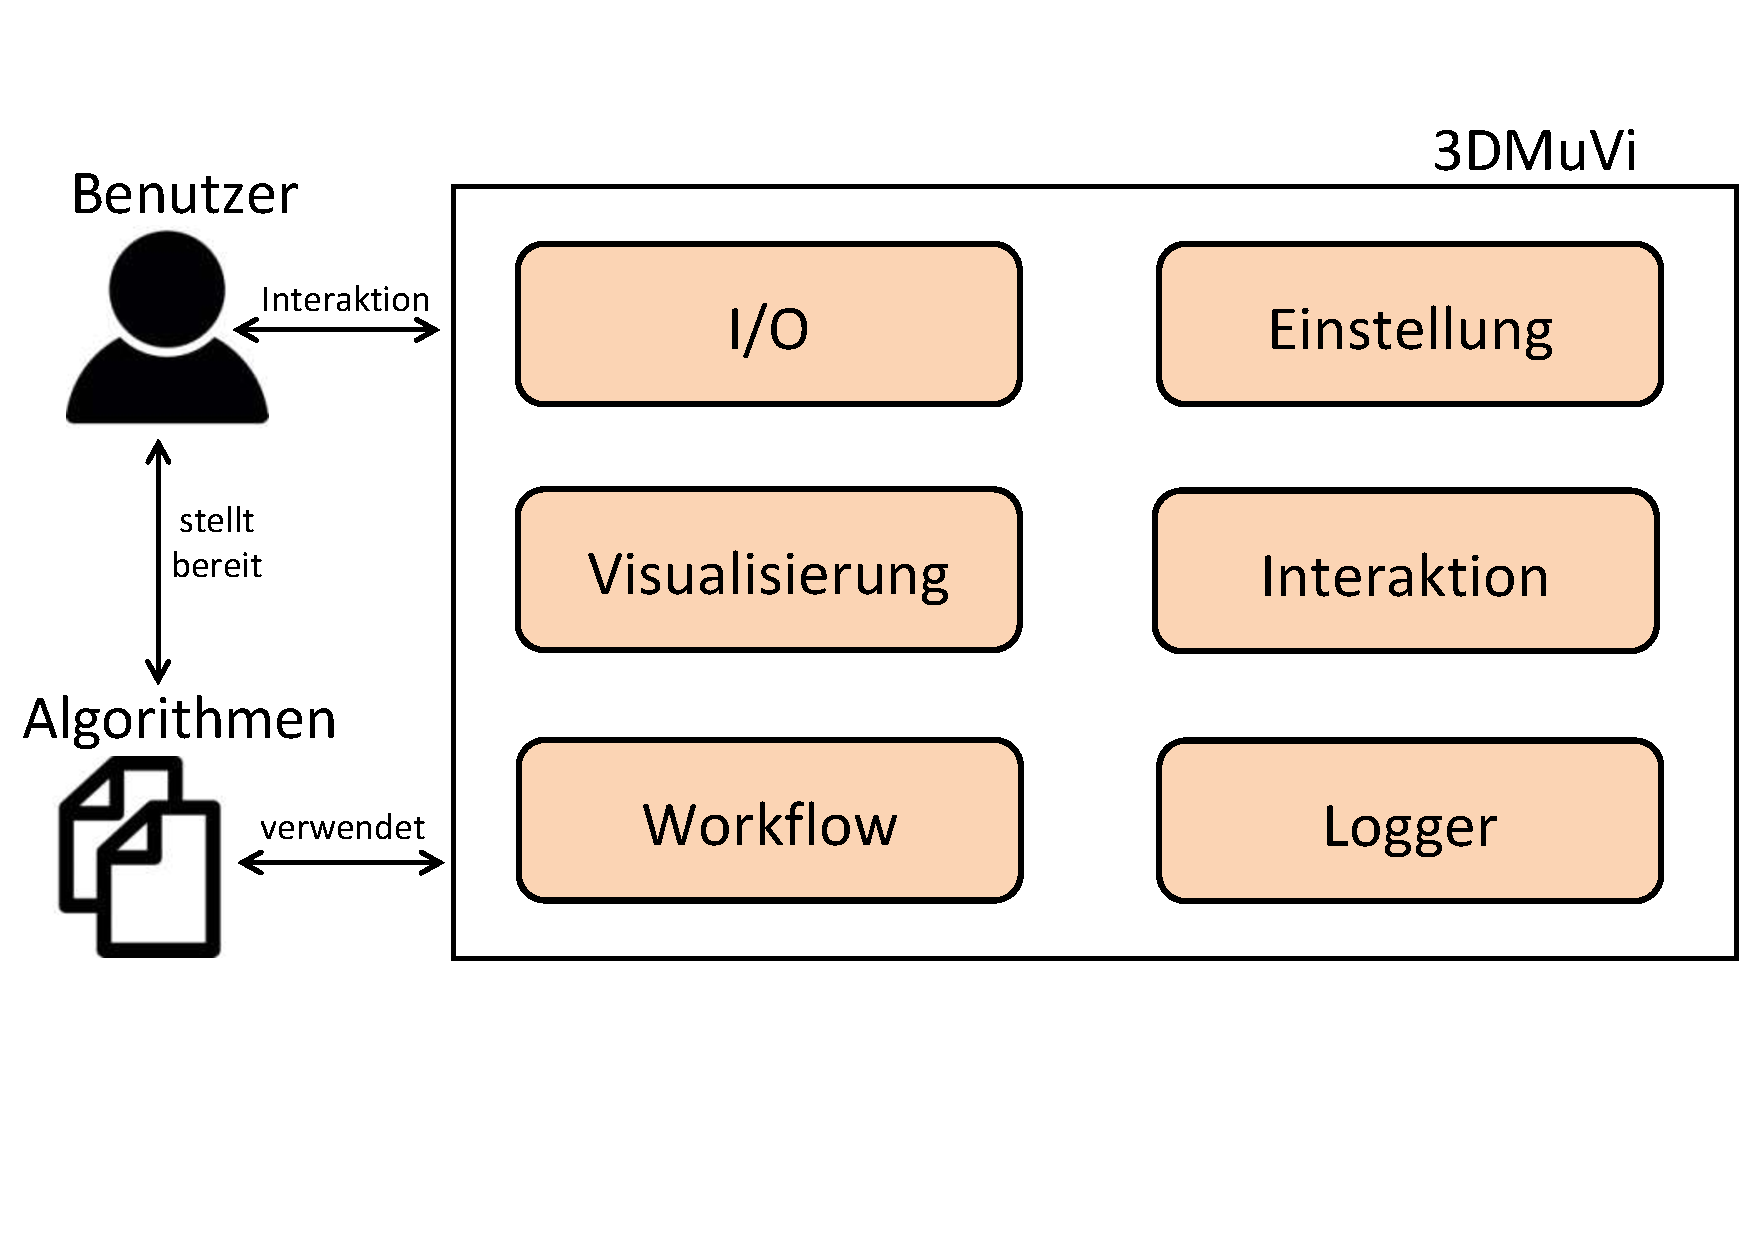
\includegraphics[width=1\textwidth]{img/SUebersicht.pdf}

\section{Module}
Im weiteren folgt eine kurze Zusammenfassung der Module.

\subsection{Workflow}
Das Modul Workflow bietet mindestens einen Workflow an und bündelt alle workflowspezifischen
Einstellungen und Auswahlmöglichkeiten, inklusive:

\begin{itemize}
\item Workflows wie den 4-Phasen-Workflow
\item Speichern und laden von Wokflowkonfigurationen
\item Algorithmenauswahl für jede Phase 
\end{itemize}

\subsection{I/O}

Das Modul I/O bietet Funktionen für die Ein- und Ausgabedaten an, inklusive:

\begin{itemize}
\item Einlesen und übergeben von Einzelbilder
\item Speichern von (Zwischen-) Ergebnissen
\end{itemize}

\subsection{Visualisierung}
Das Modul Visualisierung bietet Anzeigen der (Zwischen-) Endergebnissen  an, inklusive:

\begin{itemize}
\item Anzeigen der Ausgabedaten der (Zwischen-) Ergebniss
\end{itemize}

\subsection{Logger}
Das Modul Logger stellt Logs bereit, inklusive:

\begin{itemize}
\item Info, Warning, Error, Debug
\item Anzeige und Abspeichern dieser Logs
\end{itemize}

\subsection{Einstellung}
Das Modul Einstellungen behandelt (globale) lokale Einstellungen, inklusive:

\begin{itemize}
\item Speichern und Laden von Einstellungen einzelner Verfahren
\end{itemize}

\subsection{Interaktion}
Das Modul Interaktion behandelt Benutzereingaben innerhalb des Programms, inklusive:

\begin{itemize}
\item Starten und Stoppen, Arbeitsindikator 
\item optional, Manipulation der Ausgangsdaten der (Zwischen-) Ergebnisse
\end{itemize}

\section{Produktdaten}
Im folgenden werden alle Daten gelistet, welche abgespeichert werden.
\subsection{Daten der obligatorischen Funktionen}
\begin{enumerate}[align=left,leftmargin=4em, label={\textbf{\textbackslash PD10\arabic*0\textbackslash}} ]
	\item Zwischenergebnisse
	\item Endergebnis
	\item Parameter der einzelnen Algorithmen
\end{enumerate}
\subsection{Daten der optionalen Funktionen}
\begin{enumerate}[align=left,leftmargin=4em, label={\textbf{\textbackslash PD20\arabic*0\textbackslash}} ]
	\item Globale Einstellungen
	\item Konfiguration des Workflows
	\item Speichern weiterer Workflows
\end{enumerate}	

\section{Schnittstellen}
Hier werden die vom Programm bereitgestellten Schnittstellen beschrieben
\begin{enumerate}[ align=left, label={\textbf{\textbackslash S1\arabic*0\textbackslash}}]
\item (Funktionale-) Schnittstellen zum Aufrufen und Datenaustausch der Algorithmen
\item  Schnittstelle zum Einstellen der Algorithmen
Angabe der Config Datei und direkte Angabe eines Parameter-Trees
\end{enumerate}
\newpage 
\section{Datenflussübersicht}

Dieses Diagramm stellt eine Grobübersicht über den Datenfluss zwischen den einzelnen Modulen dar.
Diese sind nur als grobe Orientierung anzusehen und werden im Entwurf und in der Implementierung möglicherweise auf andere Weise umgesetzt.
\begin{normalsize}

\end{normalsize}
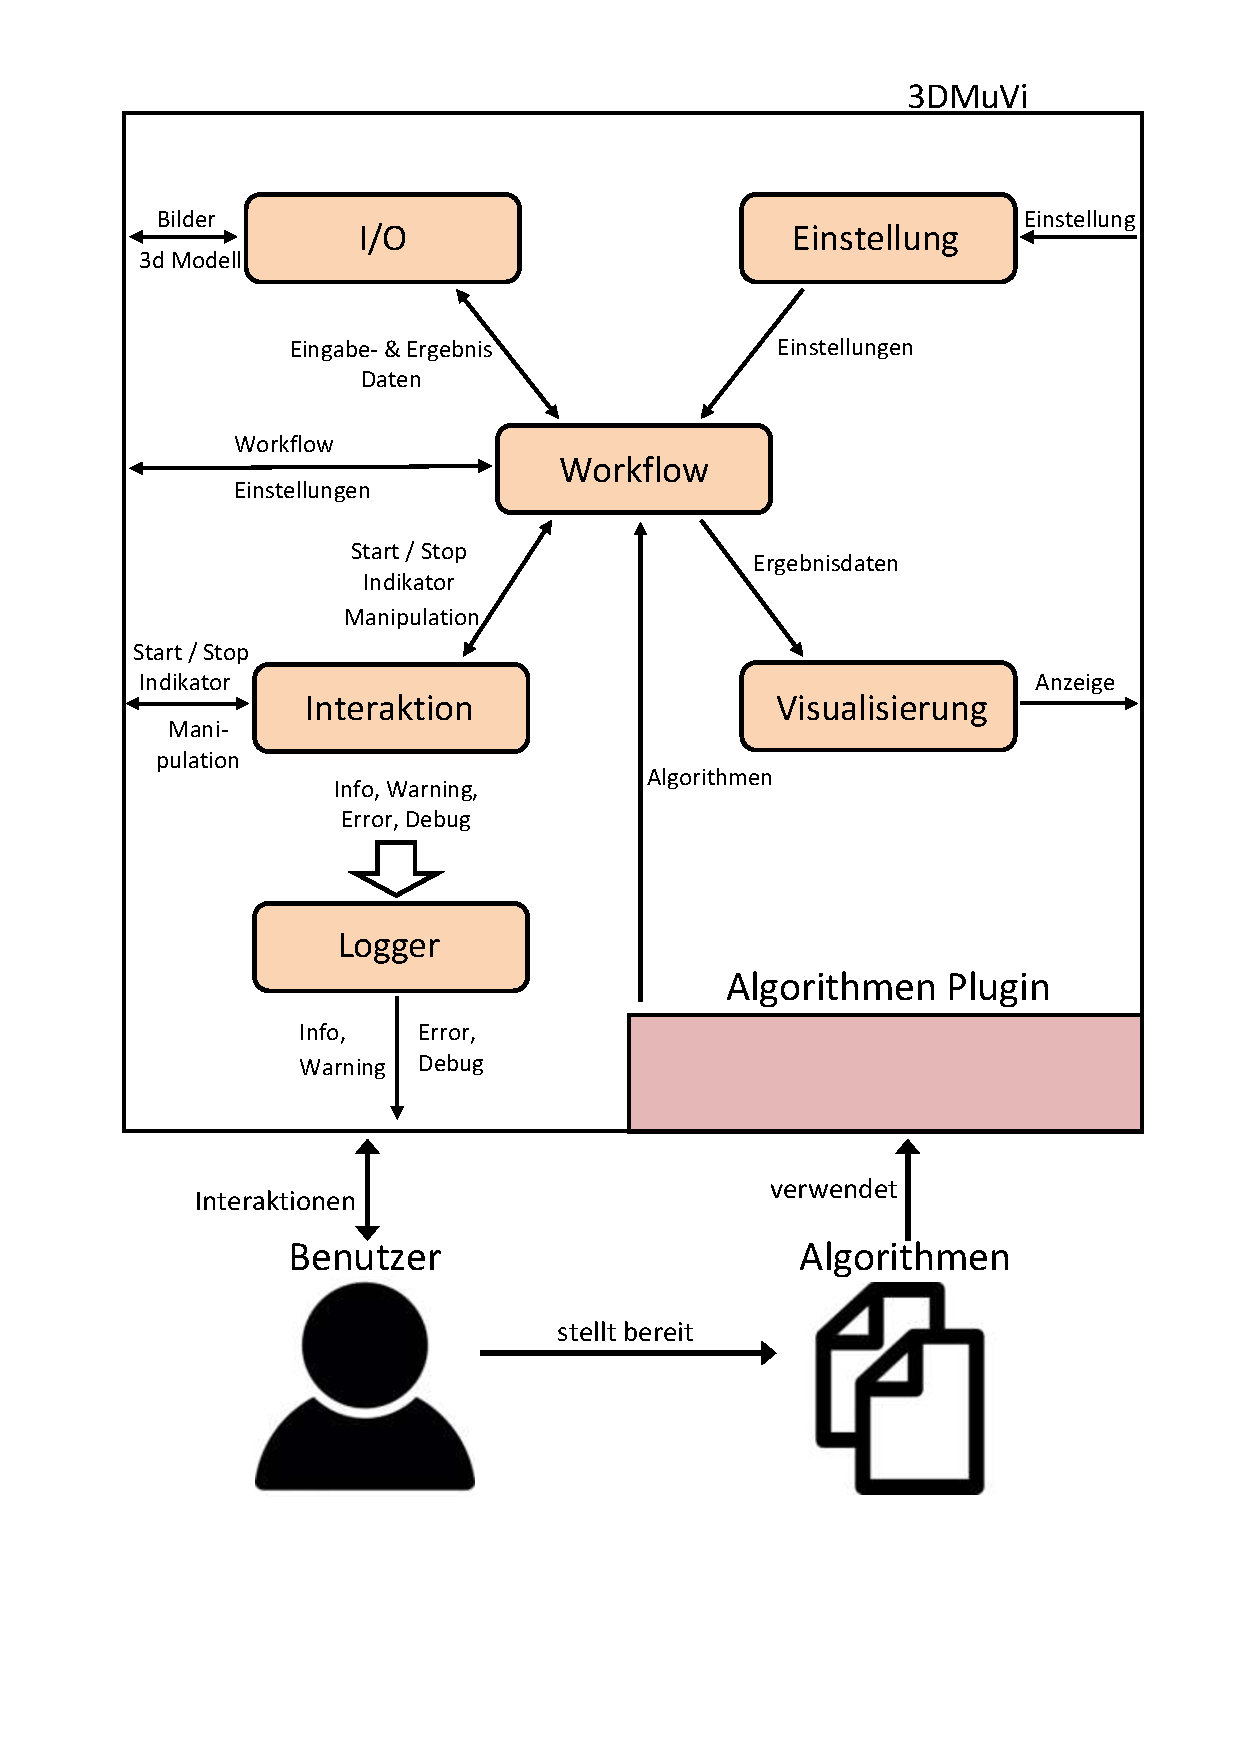
\includegraphics[width=0.87\textwidth]{img/Datenflussuebersicht.pdf} 
\newpage
 
\section{Anwendugsfälle}

\subsection{Anwendugsfall: Rekonstruktion aus unzusammenhängenden Einzelbilder}

\textbf{Gegeben:}\newline
Vielzahl an Einzelbilder einer Szene die nicht von der selben Kamera oder Position aufgenommen wurden.\newline
\textbf{Ziel:}\newline
Rekonstruktion der Szene oder eines einzelnen Objektes.\newline
\textbf{Vorgehen:}
\begin{enumerate}
\item Feature Detektor: In den Bildern wird automatisch nach „markanten“ Punkten gesucht, die hohen Wiedererkennungswert haben.\item Feature Matching: Die gefundenen „markanten Punkte“ in zwei Bildern werden verglichen und einander zugeordnet.\item Posenschätzung: Aus den Punktzuordnungen von zwei oder mehr Bildern werden die Positionen der Kameras ermittelt, von denen aus die Bilder aufgenommen wurden.\item Tiefenschätzung: Mit Hilfe der Kamerapositionen werden die Tiefen in den Bildern trianguliert. Dadurch werden die Entfernungen der Objekte auf den Bildern bestimmt.\item Modellerzeugung: Die Einzelansichten werden zu einem kompletten 3D Modell zusammengesetzt.
\end{enumerate}
\textbf{Stellschrauben:}
\begin{enumerate}
\item Der Feature Detektor kann ausgewechselt werden (z. B. SIFT oder SURF)\item Das Feature Matching kann auf verschiedene Arten durchgeführt werden (z. B. RANSAC oder MLESAC, jeweils mit verschiedener Initialisierungen)
\end{enumerate}

 
\subsection{Anwendugsfall: Structure-from-Motion (SfM)}

\textbf{Gegeben:}\newline
Videosequenz einer Szene, mit eigenbewegung der Kamera.\newline
\textbf{Ziel:}\newline
Rekonstruktion der Szene oder eines einzelnen Objektes.\newline Structure-from-Motion (SfM) ist ein Verfahren zur 3D-Rekonstruktion mit nur einer Kamera. Dabei wird bei SfM das 3D-Modell aus einem Video, also einer Reihe von Einzelbildern rekonstruiert. Dabei ist es wichtig, dass das Video nicht von einer statischen Position aus aufgenommen wird, vielmehr sollte die Kamera sich dabei mit Blick auf die zu rekonstruierende Szene bewegen. Bei der Rekonstruktion mittels SfM werden zwei oder mehr Einzelbilder der Eingangssequenz herangezogen, für die angenommen wird, dass sie dieselbe Szene aus verschiedenen Blickrichtungen betrachten und die Szene zwischen den Einzelbildern statisch (unverändert) geblieben ist.\newline
\textbf{Vorgehen:}
\begin{enumerate}
\item Feature Detection: Ermitteln leicht verfolgbarer markanter Bildpunkte\item Feature Tracking: Verfolgen der markanten Bildpunkte\item Posenschätzung: Bestimmen der Aufnahmepunkte, Verfolgen der Kamerafahrt\item Tiefenschätzung: Bestimmen der Tiefe mit lokalen Optimierungsverfahren\item Modellerzeugung: Die Einzelansichten werden zu einem kompletten 3D Modell zusammengesetzt
\end{enumerate}

\section{Typische Nutzungsabläufe}
\label{ch:usecases}
In diesem Abschnitt werden typische Abläufe von Aktionen dargestellt, die ein Anwender mit der Software durchführt.
\subsection{Laden von Einzelbildern}
\label{usecase:1}
\usecase{1}
\subsection{Auswählen von Algorithmen}
\label{usecase:2}
\usecase{2}
\subsection{Ändern von Einstellungen}
\label{usecase:3}
\usecase{3}
\subsection{Speichern der Einstellungen}
\label{usecase:4}
\usecase{4}
\subsection{Laden von Einstellungen}
\label{usecase:5}
\usecase{5}
\subsection{Öffnen der Hilfe}
\label{usecase:6}
\usecase{6}
\subsection{Filtern der Logs}
\label{usecase:7}
\usecase{7}
\subsection{Ausführen von Algorithmen}
\label{usecase:8}
\usecase{8}
\subsection{Unterbrechen der Verarbeitung}
\label{usecase:9}
\usecase{9}
\subsection{Vorschau der Ergebnisse}
\label{usecase:10}
\usecase{10}


\iffalse
\subsection{Erzeugung eines 3D-Modells}
\textbf{Vorbedingung:} Bilder des Modells wurden erstellt. \newline
\textbf{Ergebnis:} Fertiges 3D-Modell liegt zur weiteren Verarbeitung in anderer Software vor. \newline
Der Nutzer führt folgende Schritte aus (Schritte \ref{TN3DModellBilderauswahl} bis \ref{TN3DModellSpeichern} werden in 3D-MuVi ausgeführt):
\begin{enumerate}
	\item 3D-MuVi wird gestartet.
	\item \label{TN3DModellBilderauswahl} Bilder werden ausgewählt.
	\item Algorithmen für die folgenden Verarbeitungsschritte werden jeweils nacheinander ausgewählt:
	\begin{itemize}
		\item Feature Extraktion / Matching
		\item Posenschätzung
		\item Tiefenschätzung
		\item 3D Fusion
	\end{itemize}
	\item Button zum Starten der Verarbeitung wird gedrückt.
	\item \label{TN3DModellSpeichern} Ergebnisdaten werden abgespeichert.
	\item Kopieren des 3D-Modells aus dem Verzeichnisbaum der Ergebnisse an den gewünschten Ort.
\end{enumerate}

\subsection{Evaluierung von Algorithmen für Feature Extraktion / Matching}
\label{TNEvalAlgo}
\textbf{Vorbedingung:} Bilder eines Modells wurden erstellt. \newline
\textbf{Ergebnis:} Der Nutzer kann anhand der visuellen Betrachtung der Resultate einschätzen, welcher der beiden getesteten Algorithmen sich für die gewählten Bilder besser eignet. \newline
Der Nutzer führt folgende Schritte aus (Alle Schritte ab \ref{TNEvalAlgoBilderAuswahl} werden in 3D-MuVi ausgeführt):
\begin{enumerate}
	\item 3D-MuVi wird gestartet.
	\item \label{TNEvalAlgoBilderAuswahl} Bilder werden ausgewählt.
	\item Algorithmen für die folgenden Verarbeitungsschritte werden jeweils nacheinander ausgewählt:
	\begin{itemize}
		\item Feature Extraktion / Matching
		\item Posenschätzung
		\item Tiefenschätzung
		\item 3D Fusion
	\end{itemize}
	\item Button zum Starten der Verarbeitung wird gedrückt.
	\item Betrachtung der Ergebnisse.
	\item Anderer Algorithmus für den Verarbeitungsschritt Feature Extraktion / Matching wird ausgewählt.
	\item Button zum Starten der Verarbeitung wird gedrückt.
	\item Erneute Betrachtung der Ergebnisse.
\end{enumerate}

\subsection{Überprüfen des Logs von Algorithmen}
\textbf{Vorbedingung:} Bilder eines Modells wurden erstellt. \newline
\textbf{Ergebnis:} Der Nutzer kann anhand der Meldungen im Log die Eignung der gewählten Algorithmen für die Bilder einschätzen und Verbesserungen an den Algorithmen vornehmen. \newline
Der Nutzer führt folgende Schritte aus (Schritte \ref{TNLogBilderAuswahl} bis \ref{TNLogSuchen} werden in 3D-MuVi ausgeführt):
\begin{enumerate}
	\item 3D-MuVi wird gestartet.
	\item \label{TNLogBilderAuswahl} Bilder werden ausgewählt.
	\item Algorithmen für die folgenden Verarbeitungsschritte werden jeweils nacheinander ausgewählt:
	\begin{itemize}
		\item Feature Extraktion / Matching
		\item Posenschätzung
		\item Tiefenschätzung
		\item 3D Fusion
	\end{itemize}
	\item Button zum Starten der Verarbeitung wird gedrückt.
	\item Alle Arten von Meldungen im Log werden eingeblendet.
	\item \label{TNLogSuchen} Auffälligkeiten in den Meldungen des Logs werden gesucht.
	\item Algorithmen werden bei Bedarf überarbeitet.
\end{enumerate}

\section{Typische Nutzungsabläufe mit optionalen Funktionen}

Dieser Abschnitt stellt beispielhaft typische Nutzungsabläufe dar, die möglich sind, wenn bestimmte optionalen Funktionen umgesetzt sind.

\subsection{Evaluierung eines Workflows nach Entfernung eines Features in den Zwischenergebnissen}
Dieser Nutzungsablauf ist eine Erweiterung von \ref{TNEvalAlgo}. Sinn der Erweiterung ist es dem Nutzer die Möglichkeit zu geben, das Entfernen einzelner Features zu testen, bevor er den Algorithmus entsprechend anpasst. Als optionale Funktion muss das Löschen einzelner Features in den Zwischenergebnissen und das Starten ab einem bestimmten Schritt implementiert sein. \newline
\textbf{Vorbedingung:} Bilder eines Modells wurden erstellt. \newline
\textbf{Ergebnis:} Der Nutzer kann anhand der visuellen Betrachtung der Resultate einschätzen, ob das Entfernen des Features das Endergebnis verbessert oder verschlechtert. Auf dieser Grundlage kann er über weitere Anpassungen an dem gewählten Algorithmus für die Feature Extraktion nachdenken. \newline
Der Nutzer führt folgende Schritte aus (Alle Schritte ab \ref{TNOFeatureEntfBilderAuswahl} werden in 3D-MuVi ausgeführt):
\begin{enumerate}
	\item 3D-MuVi wird gestartet.
	\item \label{TNOFeatureEntfBilderAuswahl} Bilder werden ausgewählt.
	\item Algorithmen für die folgenden Verarbeitungsschritte werden jeweils nacheinander ausgewählt:
	\begin{itemize}
		\item Feature Extraktion / Matching
		\item Posenschätzung
		\item Tiefenschätzung
		\item 3D Fusion
	\end{itemize}
	\item Button zum Starten der Verarbeitung wird gedrückt.
	\item Betrachtung der Ergebnisse.
	\item In den Ergebnissen der Feature Extraktion wird ein Feature entfernt.
	\item Button zum Starten der Verarbeitung ab dem Schritt Posenschätzung wird gedrückt.
	\item Erneute Betrachtung der Ergebnisse.
\end{enumerate}

\subsection{Evaluierung von Algorithmen für Feature Extraktion / Matching auf mehreren Datensätzen}
Dieser Nutzungsablauf ist eine Erweiterung von \ref{TNEvalAlgo}. Sinn der Erweiterung ist es dem Nutzer die Möglichkeit zu geben, Workflows schnell auf mehreren Sätzen von Bildern zu evaluieren. Als optionale Funktion muss das Erstellen und Auswählen mehrerer Datensätze umgesetzt sein.\newline
\textbf{Vorbedingung:} Bilder zweier Modelle wurden erstellt (nachfolgend als Modell1 und Modell2 bezeichnet). \newline
\textbf{Ergebnis:} Der Nutzer kann anhand der visuellen Betrachtung der Resultate einschätzen, welcher der beiden getesteten Algorithmen sich für die gewählten Bilder von Modell1 bzw. Modell2 besser eignet. \newline
Der Nutzer führt folgende Schritte aus (Alle Schritte ab \ref{TNOEvalAlgoBilderAuswahl1} werden in 3D-MuVi ausgeführt):
\begin{enumerate}
	\item 3D-MuVi wird gestartet.
	\item \label{TNOEvalAlgoBilderAuswahl1} Bilder von Modell1 werden ausgewählt.
	\item Algorithmen für die folgenden Verarbeitungsschritte werden jeweils nacheinander ausgewählt:
	\begin{itemize}
		\item Feature Extraktion / Matching
		\item Posenschätzung
		\item Tiefenschätzung
		\item 3D Fusion
	\end{itemize}
	\item Button zum Starten der Verarbeitung wird gedrückt.
	\item Betrachtung der Ergebnisse.
	\item Neuer Datensatz für Modell2 wird erstellt und ausgewählt.
	\item Bilder von Modell2 werden ausgewählt.
	\item Button zum Starten der Verarbeitung wird gedrückt.
	\item Betrachtung der Ergebnisse.
	\item Anderer Algorithmus für den Verarbeitungsschritt Feature Extraktion / Matching wird ausgewählt.
	\item Button zum Starten der Verarbeitung wird gedrückt.
	\item Betrachtung der Ergebnisse.
	\item Datensatz von Modell1 wird gewählt.
	\item Betrachtung der Ergebnisse.
\end{enumerate}
\fi
	\chapter{Produktleistungen}
		% Wenn vorhanden, Anforderungen an Laufzeitverhalten oder Speicherplatz.
\section{Laufzeitverhalten}
Das Konfigurieren und Vorbereiten der Software auf das Ausführen der Algorithmen und das Anzeigen der Ergebnisse erfolgt in Echtzeit. Verzögerungen entstehen lediglich beim Ausführen des Workflows und werden dabei maßgeblich von den verwendeten Algorithmen vorgegeben. 
\section{Speicherplatzbedarf}
Für die Anwendung wird kaum Festplattenspeicher benötigt, da nur die Einstellungen der Verfahren lokale gespeichert werden. Der Hauptspeicher wird der Anwendung selbst kaum benötigt und hauptsächlich von den als Plugins implementierten Algorithmen in Anspruch genommen.
	\chapter{Benutzeroberfläche}
		% Beschreibung der anvisierten Bedienoberfläche (z.B. durch einen Prototyp oder frei gezeichnet) und Erläuterung der Menüstruktur.

\section{Hauptfenster}

\begin{figure}[h]
	\centering
	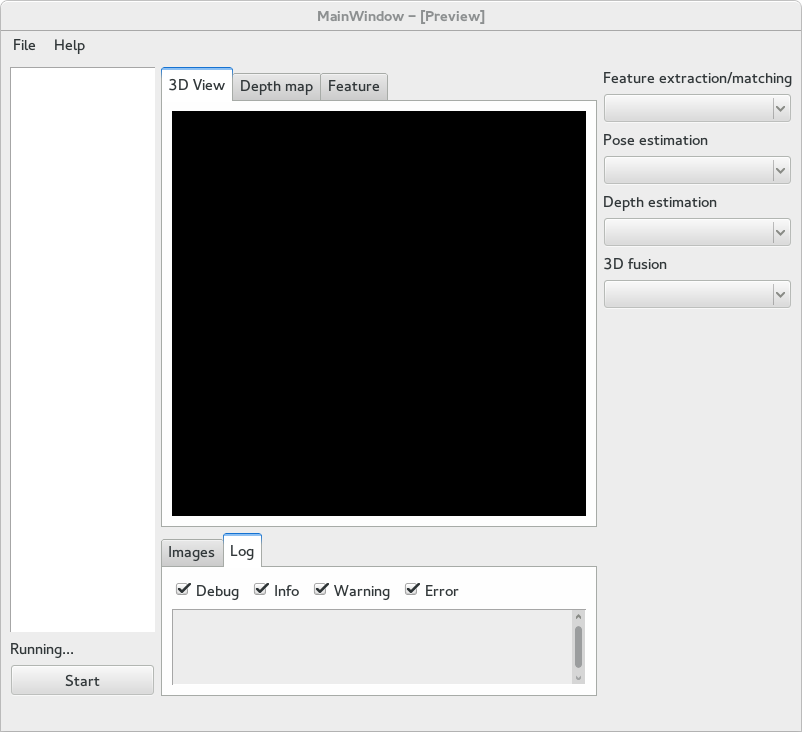
\includegraphics[width=0.9\textwidth]{img/Screenshot.png}
	\caption{Hauptfenster}
	\label{c:Hauptfenster}
\end{figure}

\begin{description}
	\item[Algorithmuswahl] Algorithmen können dem Workflow entsprechend aus ComboBoxen gewählt werden.
	\item[Bilderinput] Eingabebilder werden als Thumbnails angezeigt.
\end{description}
	\chapter{Globale Testfälle}
		% Testfälle  für  die  einzelnen  Produktfunktionen,  die  alle  abgedeckt  sein müssen. Testszenarien für typische Anwendungsszenarien.
Die Testfälle und Testszenarien dienen der Überprüfung der Software bezüglich ihrer Funktionalität und Konsistenz. Testfälle unterscheiden sich von den Testszenarien darin, dass diese automatisierte, somit atomare Funktionstests darstellen, während Testszenarien manuelle Testanweisungen sind, die durch eine ungeschulte Testperson durchgeführt werden sollen.

\section{Testfälle}
Die Testfälle sind alle Automatisiert und werden mit der in Qt integrierten Test-Suite durchgeführt.
\subsection{Funktionstests}
Zuerst wird jede Klasse einzeln bearbeitet. Jede Öffentliche Methode wird mit zwei Testfällen getestet. Der erste Testfall testet das Verhalten einer Funktion im normalen Umfeld mit gewöhnlichen Parametern. Dieser Test dient dazu, Fehler in Berechnungsvorschriften und Implementierungen zu finden. Der zweite Testfall ruft die Funktion mit ungewöhnlichen Parametern auf, eventuell auch mit falschen Datentypen. Diese Tests dienen dazu, die Robustheit der Funktionen zu garantieren. Die Argumente, die an eine Funktion übergeben werden, sind so weit wie möglich Zufällig verteilt zu wählen. Für das nachvollziehen von Fehlern werden die getesteten Parameter zusätzlich zu der Fehlerbeschreibung ausgegeben.
\subsection{Komponententests}
Komponententests testen das Verhalten eines isolierten Moduls der Anwendung. Viele der Tests lassen sich allerdings erst nach der Entwurfsphase festlegen, weshalb dieser Abschnitt bis zum Vollständigen Entwurf der Anwendung noch nicht vollständig sein wird.

	\begin{enumerate}[align=left, leftmargin=4em, label={\textbf{\textbackslash T2.\arabic*0\textbackslash}} ]
		\item \begin{tabular}{|c|c|}
			\hline Modul & Funktion \\ 
			\hline I\textbackslash O & FM210 \\ 
			\hline 
		\end{tabular}\\ 
		\subitem \textbf{Ziel:}\\ Testen der Funktionalität Laden und Weitergeben von Eingabebildern.
		\subitem \textbf{Dummies:} \begin{itemize}
			\item Algorithmus, der die empfangenen Bilder an den Test meldet.
			\item Interaktion, die das Modul mit vordefinierten Bildern versorgt.
		\end{itemize}
		\subitem \textbf{Erwartetes Verhalten:}\\
		Die vom Algorithmus gemeldeten Bilder entsprechen den Bildern, die dem Modul übergeben wurden.
		
		\item \begin{tabular}{|c|c|}
			\hline Modul & Funktion \\
			\hline I\textbackslash O & FM220 \& FM230 \\
			\hline
		\end{tabular}\\
		\subitem \textbf{Ziel:}\\ Testen der Fähigkeit, Zwischenergebnisse strukturiert abzuspeichern.
		\subitem \textbf{Dummies:} \begin{itemize}
			\item Algorithmen, die Zufällig verteilte Zwischenergebnisse liefern, deren Art und Typ nicht weiter Definiert ist.
		\end{itemize}
		\subitem \textbf{Erwartetes Verhalten:}\\
		Es wird eine Ordnerstruktur in dem vom Test vorgegebenen Verzeichnis angelegt mit den gespeicherten Daten.
		\item \begin{tabular}{|c|c|}
			\hline Modul & Funktion \\
			\hline Logger & FM410 \\
			\hline
		\end{tabular}\\
		\subitem \textbf{Ziel:} \\ Testen der Logfunktionalität
		\subitem \textbf{Dummies:} \begin{itemize}
			\item Generator von Lognachrichten
		\end{itemize}
		\subitem \textbf{Erwartetes Verhalten:}\\
		Nach dem Anlegen der Logs und dem auswählen der einzelnen Loglevel werden nur Nachrichten des gewählten Loglevels zurückgegeben.
		\item \begin{tabular}{|c|c|}
			\hline Modul & Funktion \\
			\hline Logger & FM410 \\
			\hline
		\end{tabular}\\
		\subitem \textbf{Ziel:} \\ Testen der Speicherfunktionalität
		\subitem \textbf{Dummies:} \begin{itemize}
			\item Generator von Lognachrichten
		\end{itemize}
		\subitem \textbf{Erwartetes Verhalten:}\\
		Nach dem Anlegen der Logs und dem Abspeichern wird eine Datei an dem spezifizierten Pfad vorgefunden.
		\item \begin{tabular}{|c|c|}
			\hline Modul & Funktion \\
			\hline Einstellungen & FM510 \\
			\hline
		\end{tabular}\\
		\subitem \textbf{Ziel:} \\ Test der Einstellungen für Algorithmen
		\subitem \textbf{Dummies:} \begin{itemize}
			\item Algorithmus, der eine Liste von Einstellungen bereitstellt, welche alle Datentypen abdeckt und bei Variationsmöglichkeiten der Typen bzw. Wertebereiche diese Stichprobenartig vorhanden sind.
		\end{itemize}
		\subitem \textbf{Erwartetes Verhalten:}\\
		Nach dem Abspeichern findet sich eine Datei an dem spezifizierten Pfad. Nach dem Laden dieser Datei enthält ein neu Instantiierter Algorithmus dieselben Einstellungen wie der erste Algorithmus, welcher zur Speicherung verwendet wurde.
		\item \begin{tabular}{|c|c|}
			\hline Modul & Funktion \\
			\hline Einstellungen & FK410 \\
			\hline
		\end{tabular}\\
		\subitem \textbf{Ziel:} \\ Test der Einstellungen für Globale Parameter
		\subitem \textbf{Dummies:} \begin{itemize}
			\item Keine
		\end{itemize}
		\subitem \textbf{Erwartetes Verhalten:}\\
		Nach dem Sichern globaler Einstellungen findet sich eine Datei an dem spezifizierten Pfad. Nach dem Lesen dieser Datei in eine neue Einstellungs-Instanz enthält diese dieselben Daten wie die Instanz, die zur Speicherung verwendet wurde.
		\item \begin{tabular}{|c|c|}
			\hline Modul & Funktion \\
			\hline Workflows & FK230 \\
			\hline
		\end{tabular}\\
		\subitem \textbf{Ziel:}\\ Testen des Abspeicherns von Workflow-Konfigurationen
		\subitem \textbf{Dummies:} \begin{itemize}
			\item Keine
		\end{itemize}
		\subitem \textbf{Erwartetes Verhalten:}\\ Nach dem zufälligen Zusammenbau eines Workflows kann dieser in eine Datei gesichert werden und entspricht nach dem laden dem gesicherten Workflow.
		\item \begin{tabular}{|c|c|}
			\hline Modul & Funktion \\
			\hline Interaktion & FK310 \\
			\hline
		\end{tabular}\\
		\subitem \textbf{Ziel:}\\ Testen des Ladens von Zwischenergebnissen
		\subitem \textbf{Hinweis:}\\ Wenn die Funktionalität implementiert wird, muss dieser Test mit dem Test \textbackslash T2.20\textbackslash zusammengeführt werden.
		\subitem \textbf{Dummies (Ergänzung):}\begin{itemize}
			\item Ein Algorithmus, der die Ausgabe des ersten Algorithmus als Eingabe nimmt und ihre Validität prüft.
		\end{itemize}
		\subitem \textbf{Erwartetes Verhalten (Ergänzung):}\\ Nach dem Laden der Zwischenergebnisse kann der zweite Algorithmus die Daten erfolgreich Validieren.
		\item \begin{tabular}{|c|c|}
			\hline Modul & Funktion \\
			\hline Foo & Bar \\
			\hline
		\end{tabular}\\
		\subitem Platzhalter für weitere Komponententests
	\end{enumerate}

\section{Testszenarien}
	\begin{itemize}
		\item \textbf{Testszenario 1}\\
		Blub
	\end{itemize}
	\chapter{Qualitätszielbestimmungen}
		% Anforderungen  an  Stabilität,  Robustheit,  Leistungsfähigkeit  etc.  des Systems.  Dies  beinhaltet  auch  den  Umgang  mit  fehlerhaften  Eingabedaten  oder  fehlerhaften Konfigurationen.
\section{Übersicht}
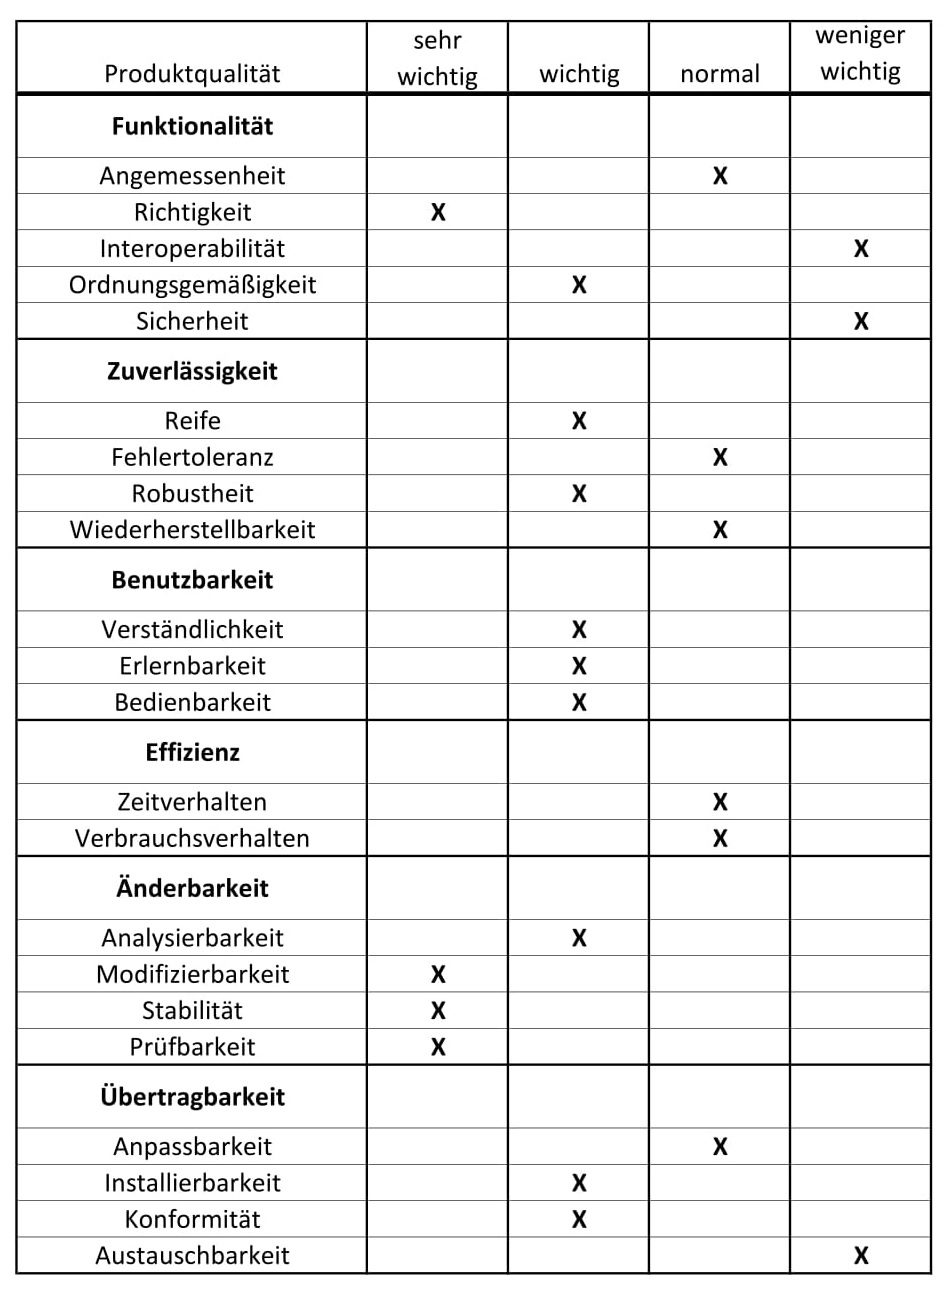
\includegraphics[scale=0.5]{img/Quali.jpg} 
\section{Zusammenfassung}
\begin{itemize}
\item Der Hautfokus der Software liegt auf korrekter Funktionsweise und Erweiterungen mit Hilfe von Plugins (Hauptsächlich weitere Algorithmen und Workflows).  
\item wichtige Qualitätsmerkmale sind gute Bedienbarkeit bei fachlichem Verständnis und Zuverlässigkeit, solange funktionstüchtige Algorithmen verwendet werden. Außerdem soll das Programm ohne großen Aufwand auf einem Linux-System installierbar sein.
\item Die Effizienz des Programms ist kaum beeinflussbar, da sie hauptsächlich von den verwendeten Algorithmen und Parametern dieser abhängt.
\item Sicherheit, Interoperabilität und Austauschbarkeit werden als weniger wichtig erachtet, da das Programm eigenständig und auf einzelnen Computern ausgeführt wird.
\end{itemize}
	\chapter{Entwicklungsumgebung}
		% Zur Entwicklung verwendete Hard‐ und Software. In der Pflichtenheft‐Phase soll  sich  das  Team  in  die  Werkzeuge  einarbeiten  und  sich  hier  vorläufig  festlegen.  Zu  diesen Werkzeugen zählen unter anderem ein UML‐Modellierungswerkzeug, IDE, Code‐Verwaltungssystem.

\section{Allgemein}
	\begin{itemize}
		\item \LaTeX
		\item Versionskontrolle (Git)
	\end{itemize}
\section{Implementierung}
	\begin{itemize}
		\item Qt Creator
		\item ...
	\end{itemize}
\section{Validierung}
	\begin{itemize}
		\item QtUnit
	\end{itemize}
\section{???}
	\begin{itemize}
		\item Bla
	\end{itemize}

	\chapter{Glossar}
		% Esentielle Begriffe.

\begin{description}
	\item[Point cloud] Menge von Punkten eines Vektorraums.
	\item[Algorithmus]
	\item[Visualisierung]
	\item[Schweregrad] Bezeichnet im Zusammenhang mit Lognachrichten deren Loglevel
\end{description}

\end{document}